\documentclass[10pt]{article}
\usepackage[a4paper, total={170mm, 257mm}]{geometry}

\usepackage[
backend=biber,
style=nature,
sorting=none
]{biblatex}
\addbibresource{References.bib}
%\bibliographystyle{unsrt}


\usepackage{amsmath}
\usepackage{amssymb}
\usepackage{upgreek}
\usepackage{dsfont}
\usepackage{esint} % various fancy integral symbols
\usepackage{mathrsfs} % for \mathscr

% fancy notation stuff
\usepackage{accents}
% vector arrows under the symbol to distinguish covariant and contravariant
\newcommand\undervec[1]{\underaccent{\vec}{#1}}

\usepackage{siunitx}
\DeclareSIUnit{\litre}{l} % litres as lower case l (upper case L by default)

%\usepackage{hyperref}

\usepackage{graphicx} % Required for inserting images
\usepackage{multicol}
\usepackage{mathpazo}
\usepackage[font=sf,labelfont=bf]{caption}

% title, headings, abstract heading in sans serif font and maybe color
%\usepackage{sectsty}
%\usepackage{titling}
%\usepackage[sf,bf,pagestyles]{titlesec}
\usepackage[dvipsnames]{xcolor}
\usepackage{sectsty}
\usepackage{abstract}
\renewcommand\abstractnamefont{\sffamily\bfseries}%\color{Maroon}}
%\chapterfont{\color{blue}}  % sets colour of chapters
\sectionfont{\sffamily}%\color{Maroon}}  % sets colour of sections
\subsectionfont{\sffamily}%\color{Maroon}}  % sets colour of subsections
\subsubsectionfont{\sffamily}  % sets colour of subsections





% TO DO's
\newcommand{\todo}[1]{ {\color{ForestGreen} [#1]} }

\graphicspath{{figures/}}

\usepackage{lipsum} 

% referencing commands
\newcommand{\seefig}[2]{\mbox{\sffamily($\rightarrow$ Fig. \ref{#1}#2)}}
\newcommand{\reffig}[2]{\mbox{\sffamily{Figure \ref{#1}#2}}}


\title{\sffamily\bfseries\color{MidnightBlue} Scattering Spectroscopy of\\Plasmonic Janus Particles\\\mbox{ }\\Supplementary Material}
\author{Felix H. Patzschke and *Frank Cichos}
%\date{November 2023}
\date{}



\begin{document}
%\allsectionsfont{\sffamily}

\maketitle

\sectionfont{\sffamily\color{MidnightBlue}}  % sets colour of sections
\subsectionfont{\sffamily\color{MidnightBlue}}  % sets colour of subsections



\section*{Orientation Definition}
The orientation of the system is characterised by the angles between three unit vectors;
\begin{itemize}
    \item[$\hat{k},$] the propagation direction of the incident light, with respect to which scattering angles are defined, 
    \item[$\hat{o},$] the "forward" direction along the optical axis, equivalent to the central axis of the objective's collection cone and
    \item[$\hat{z},$] the symmetry axis of the particle, oriented such that the Au cap lies in the positive and the PS side in the negative $z$-direction.
\end{itemize}
In terms of these, the out-of-plane orientation of the JP is defined as
$\alpha := \measuredangle( \hat{o}, \hat{z} )$.
Similarly, we define the illumination angle 
$\zeta := \measuredangle( \hat{k}, \hat{z} )$, 
which, in this model, is the only orientation parameter needed to define the light-matter interaction of the JP. 

Scattering angles are defined for each plane-wave contribution to the scattered field: 
Let that contribution have a propagation direction $\hat{k}'$. 
Then, \mbox{$\theta := \measuredangle( \hat{k}', \hat{k} )$} is the polar component of the scattering angle. 
Additionally, there is an azimuthal component $\phi$, the choice of reference point for which being somewhat arbitrary. 
In the following, it will be chosen such that if $\hat{k}'$ lies in the $(\hat{k},\hat{z})$ plane, then $\phi=0$.

These definitions are illustrated in \reffig{fig:vectors-and-angles}{}.  

\begin{figure}[htbp]
    \centering
    \begin{overpic}[width=0.5\columnwidth]{angles_sketch_larger_v2}
    % subplot label
    %\put (0,96) {{\sffamily\textbf{A}}}
    % vector labels
    \put (44,4) {$\hat{o}$}
    \put (0,31.5) {\textcolor{ts_y}{$\hat{z}$}}
    \put (0,67.5) {\textcolor{ts_b}{$\hat{k}_0$}}
    \put (77,6) {\textcolor{ts_r}{$\hat{k}'$}}
    % angle labels
    \put (60,74.5) {\textcolor{ts_b}{$\zeta$}}
    \put (33.5,27) {\textcolor{ts_y}{$\alpha$}}
    \put (30,80
    ) {{$\theta_o$}}
    \put (69,32) {\textcolor{ts_r}{$\theta$}}
    \end{overpic}
    \caption{
        %{\sffamily\textbf{A:}} 
        Unit vectors and angles defining the orientation of the system. 
        %{\sffamily\textbf{B:}} 
        %\todo{Integration domain corresponding to the objective aperture.} 
    }
    \label{fig:vectors-and-angles}
\end{figure}





\section*{Finite-Element Simulation}



The finite-element simulations were performed in COMSOL \mbox{Multiphysics 6.1}. 
%The simulation per se is ignorant of real-world optical devices and.
%Therefore, the geometric definition of the model does not depend on \mbox{$\hat{o}$-direction} or the objective aperture. 
\todo{Reference that the COMSOL model is qualitatively the same as in \cite{BA}.} 

The model was defined as follows: 
A polystyrene (PS) sphere ($r=\SI{0.5}{\micro\meter}$), centered at the origin, represents the core of the JP. 
The gold cap is modelled as half of an ellipsoidal shell around the PS sphere, cut off in the $z=0$ plane. 
Its semi major axis is parallel to $\hat{z}$ with a length of $\SI{0.55}{\micro\meter}$, its semi minor axes with length $\SI{0.51}{\micro\meter}$ lie in the $(x,y)$ plane.\footnote{$\hat{x},\hat{y},\hat{z}$ form a right-handed orthonormal basis of $\mathds{R}^3$.} 
This gives a thickness of $\SI{50}{\nano\meter}$ at the apex and a width of $\SI{10}{\nano\meter}$ to the rim. 
%The ellipsoid is cut off in the $(x,y)$ plane of the minor axes, its major axis coincides with the symmetry axis of the JP. 
%The particle model is surrounded by an ambient medium with a constant, real-valued refractive index. 
%The model geometry, based on models E1 and E2 from \cite{BA}, was defined in particle-coordinates, i.e. $\hat{z}$ coincides with the $z$-axis and $\hat{k}$ lies in the $xz$ plane. 
\todo{sketch?}

For the complex refractive index of gold, the values by Johnson \& Christy \cite{Johnson1972} were used. 
The medium surrounding the particle was modelled with a refractive index of $1.51$ to mimic the immersion oil used in the experiments. 

As parameters, the simulation takes in the illumination angle $\zeta$ and the incident (vacuum-)wavelength $\lambda$, such that
$$
    \vec{k}_0 = \frac{2\pi \mathfrak{n}}{\lambda} \left( \cos\zeta \cdot \hat{z} + \sin\zeta \cdot \hat{x} \right)
$$
is the wave vector of the incident light field. 

Given a plane wave 
$$
    \vec{E}_\mathrm{incident}(\vec{x},t) = \vec{E}_0 \cdot \exp\!\left( \mathfrak{i}\ \vec{k}_0\cdot\vec{x} - \mathfrak{i}\ \omega\ t \right)
$$
as the incident field, the solver produces a point-wise solution 
$$
    \vec{E}(\vec{x},t) = \vec{E}_\mathrm{incident}(\vec{x},t) + \vec{E}_\mathrm{sca}(\vec{x},t)
$$ 
to Maxwell's field equations on the defined geometry, where $\vec{E}_\mathrm{sca}(\vec{x},t)$ is the scattered field. 






The scattering cross-section of the particle was calculated from the scattered field as 
$$
    \sigma_\mathrm{sca} = \frac{2 \mu_0 \mu_r}{ {\bigl\Vert \vec{E}_0 \bigr\Vert}^2 } \cdot \oint_{\partial V} {\left\langle \vec{S}_\mathrm{sca} \right\rangle}_t \cdot\mathrm{d}\vec{A} \ ,
$$
where $\vec{S}_\mathrm{sca}$ is the Poynting vector of the scattered field and $\langle\cdot\rangle_t$ denotes the time average. 

%\todo{Explanation on how the scattering intensity is resolved for $\hat{k}$} 
The scattered field can, according to Fourier's theorem, be decomposed into plane-wave components
$$
    \mathrm{d}\vec{E}(\vec{x},t) := \vec{\mathcal{E}}(\vec{k}) 
    \cdot 
    \exp{\!\left(\mathfrak{i}\ \vec{k}\cdot\vec{x} - \mathfrak{i}\ \omega\ t \right)}
    \ \mathrm{d}^3 k
    \ , 
$$
such that $ \vec{E}_\mathrm{sca} = \iiint_{\mathds{R}^3}\,\mathrm{d}\vec{E}$. 
The amplitudes $\vec{\mathcal{E}}(\vec{k})$ of the components are given by the Fourier transform of $\vec{E}(\vec{x},t)$. 
The intensities of the components are given by \cite{Griffiths-ED,MA} 
$$
    \mathrm{d}\mathcal{I}(\vec{k}) = \frac{ 1 }{ 2\mu_0 \mu_r }\,{\left\langle {\left\Vert \vec{\mathcal{E}}(\vec{k}) \right\Vert}^2 \right\rangle}_t \ \mathrm{d}^3k
    \ .
$$

With any fixed wavelength $\lambda$, the wavevectors are conveniently expressed as $ \vec{k} = 2 \pi \lambda^{-1} \cdot \hat{k}'$, where \mbox{$\hat{k}' \in \mathcal{S}^2$} is a unit vector. 
One obtains the spectral and angular distribution of scattered light, $\mathrm{d}\mathcal{I}(\lambda, \Omega)$, where $\Omega$ parametrizes the 2-sphere. 

%Expressing $\Omega$ in spherical coordinates, we define the \emph{polar scattering angle} 
%$$
%\theta := \measuredangle \left( \hat{k}, \hat{k}_\mathrm{sca} \right)
%$$
%and the \emph{azimuthal scattering angle} $\phi$ s.t. 




\subsection*{Simulation of unpolarized light}

A plane wave, as it was used to simulate the LMI, is inherently polarized: 
$$
    \left[ \vec{E}_\mathrm{incident} \left[ \lambda, \zeta \right] \right] (\vec{x}, t) = \vec{E}_0 \cdot \exp\!\left( \mathfrak{i}\ \vec{k}_0\cdot\vec{x} - \mathfrak{i}\ \omega\ t \right)
$$
In contrast, measurements were conducted with unpolarized light and no polarization state was measured. 

\note{In order to get rid of the inherent polarization, ...}

For each fixed tuple of parameters, we simulated the system twice, the difference being the polarization of the incident plane wave: 
$$ \vec{E}_{0,xz} \perp \vec{E}_{0,y} $$
Then, we computed values of time-averaged observables (like scattering intensities and cross-sections) as 
$$ X_\mathrm{average} = \frac{ X_{xz} + X_{y} }{2} \ . $$ 






\section*{Selective Integration}

%In order to be able compare the simulation results to the measurements, the the limited collection angle of the objective has to be taken into account. 

In the experiment, scattered light can only contribute to recorded scattering signals if it is collected by the objective. 
While the "true" scattering intensity is the integral over the angular distribution of scattered light, 
$$
    I_\mathrm{sca}(\lambda) = \oiint_{\mathcal{S}^2} \,\mathrm{d}\mathcal{I}(\lambda, \Omega) \ , % \ \mathrm{d}\Omega \ ,
$$
the measured value corresponds to the integration over a certain angular range, % $\mathcal{D} \subset \mathcal{S}^2$: 
$$
    I_\mathrm{sca,measured}(\lambda) = \iint_{\mathcal{D}} \,\mathrm{d}\mathcal{I}(\lambda, \Omega) \ , 
$$
where $\mathcal{D} \subseteq \mathcal{S}^2$ is the set of propagation directions $\hat{k}'$, for which a plane wave component will pass through the objective aperture. %contribute to the signal on the detector. 
Specifically, $\mathcal{D}$ is the interior of a small circle which is centered around $\hat{o}$ and whose angular radius $\rho$ is defined by the numerical aperture of the objective, 
$$
    \rho = \mathrm{asin}\!\left( \frac{\mathrm{NA}}{n_\mathrm{oil}} \right) \ ,
$$
according to the Abbe sine condition. \cite{MONA-BFP-photonic-crystals,MONA-BFP-photonic-stop-bands} \todo{Sketch!}
Analytically, this requirement can be formulated as 
$$
    \mathcal{D} = \left\lbrace\ \hat{k}' \in \mathcal{S}^2\ \middle\vert\ \measuredangle\!\left( \hat{k}', \hat{o}\right) < \rho\ \right\rbrace
    \ .
$$

%In the experiment, $\hat{o}$ and $\theta_o$ are fixed, and $\hat{k}_0$ is a known parameter. 
%In the simulation, $\hat{z}$ is fixed instead, while $\zeta$ (and thus $\hat{k}_0$) is varied. 

As the objective is not considered in the simulations of the scattering process per se, appropriate values for $\hat{o}$ and $\mathrm{NA}$ have to be chosen now, in order to emulate an experiment: 
We first choose a fixed $\alpha$ and then compute a sampling of pairs $\left( \hat{k}'_0 , \hat{o}' \right) \in \left. \mathcal{S}^2 \right\vert_{y=0} \times \mathcal{S}^2$, such that 
$$
    \measuredangle\!\left(\hat{k}'_0 , \hat{o}'\right) = \theta_0 = \mathrm{asin}\!\left( \frac{\mathrm{NA}_\mathrm{DFC}}{n_\mathrm{oil}} \right) \ , 
$$
the angle between the optical axis and the illumination cone from the dark-field condenser. 
We then choose the simulations corresponding to the illumination angles defined by $\hat{k}'_0$ and the fixed $\hat{z}$ and integrate the simulated scattering intensities over the domains $\mathcal{D}$ defined by $\hat{o}'$ and $\mathrm{NA}$, accumulating the results over all pairs $\left( \hat{k}'_0 , \hat{o}' \right)$.

The end result of the selective integration is a sampled map 
$$
    \alpha,\mathrm{NA} \mapsto \bigl[ \lambda \mapsto I_\mathrm{sca,measured} \bigr] \ ,
$$
i.e. a scattering spectrum $\lambda \mapsto I_\mathrm{sca,measured}$ as measured for each sampled $\alpha,\ \mathrm{NA}$. 

%\begin{itemize}
%    \item The simulation provides values of the scattered field for sampled values of $\zeta$.
%    \item The numerical aperture of the dark-field condenser defines $\measuredangle(\hat{k},\hat{o})$.
%    \item The out-of-plane angle $\alpha$ of the JP is unknown and not uniquely defined by $\zeta$ and $\measuredangle(\hat{k},\hat{o})$. We sample $\alpha\in\left[0,\pi\right]$ and weight the results by $p(\alpha) = \sin\alpha$.\footnote{$p(\alpha)$ is the probability density function for the out-of-plane angle of a randomly oriented spherical JP. For the derivation, see the supplementary material.}
%\end{itemize}





\section*{Integration of the Far-Field Intensities}

For a given incident wavelength and illumination angle, let the scattering intensity in the far-field be
$$I_\mathrm{far}(\theta,\phi)\ .$$
The data retrieved from the simulation are $I_n$, samples of $I_\mathrm{far}$ in points $\left( \theta_n, \phi_n \right)$ on the unit sphere $\mathcal{S}^2$. 
To compute
$$
    \iint_{\mathcal{T}} I_\mathrm{far} \ \mathrm{d}\Omega \approx \sum_{n \vert \left( \theta_n, \phi_n \right)\in\mathcal{T}} I_n \ \Delta\Omega_n \ , 
$$
we must determine the values of $\Delta\Omega_n$. [TODO: Notation]

We project the spherical coordinates $\left( \theta_n, \phi_n \right)$ into the Euclidean plane, obtaining the cartesian coordinates $(x_n, y_n)$.\footnote{The choice of projection is somewhat arbitrary, we chose the stereographic projection.} 
We then compute the Voronoi tesselation which maps each projected sample point $(x_n, y_n)$ to an area element\footnote{the fact of which being a convex polygon being computationally convenient, yet analytically irrelevant} 
$$
P_n = \left\lbrace 
(x,y) \in \mathds{R}^2 
\middle\vert 
\mathrm{arg}\min\limits_{n'} \Bigl( m_\mathrm{E}\bigl( (x,y)-(x_{n'},y_{n'}) \bigr) \Bigr)
= n
\right\rbrace
$$ 
with the Euclidean metric $m_\mathrm{E}$. 
The area elements $\Delta\Omega_n$ are then given as 
$$
\Delta\Omega_n
=
\mu\left(
P_n \cap \mathcal{T}
\right) \cdot \tau\left( \theta_n, \phi_n \right)
$$
where $\mu(\cdot)$ denotes the measure of a subset of $\mathds{R}^2$ and $\tau$ is the area element transfer function associated with the chosen projection. 





\section*{Derivation of the probability density for the out-of-plane angle}

The model JP is cylindrically symmetric. Therefore its orientation in space is completely described by the direction of its axis of symmetry, $\hat{z}$. 
For the random orientation, let $\hat{z}$ be evenly distributed over $\mathcal{S}^2$. 
For a PDF $p_\Omega$ w.r.t. the solid angle $\Omega$, this means
$$
\iint_{\mathcal{T}} p_\Omega \ \mathrm{d}\Omega
=
\frac{
\iint_{\mathcal{T}} \mathrm{d}\Omega
}{
\varoiint_{\mathcal{S}^2} \mathrm{d}\Omega
}
\quad\forall\ \mathcal{T}\subseteq\mathcal{S}^2
\ .
$$
$\varoiint_{\mathcal{S}^2} \mathrm{d}\Omega$ is nothing else than the surface area of the unit sphere, $4\pi$. 
Therefore, 
$$
\iint_{\mathcal{T}} p_\Omega \ \mathrm{d}\Omega
=
\frac{1}{4\pi}\ 
\iint_{\mathcal{T}} \mathrm{d}\Omega
\quad\forall\ \mathcal{T}\subseteq\mathcal{S}^2
\ ,
$$
which implies that
$$
p_\Omega=\frac{1}{4\pi}\ .
$$

Now, we parametrise $\mathcal{S}^2$ in spherical coordinates $(\alpha,\beta)$, where $\alpha$ is the polar coordinate and $\beta$ is the azimuthal coordinate. 
The differential solid angle is
$$
\mathrm{d}\Omega = \sin\alpha \ \mathrm{d}\alpha \ \mathrm{d}\beta \ .
$$
The PDFs w.r.t. these coordinates, $p_{\alpha}$ and $p_\beta$, must satisfy
$$
\begin{aligned}
\text{a)}&&
\int_0^\pi p_{\alpha} \ \mathrm{d}\alpha &= 1
\\
\text{b)}&&
\int_0^{2\pi} p_{\beta} \ \mathrm{d}\beta &= 1
\\
\text{and c)}&&
\iint_{\mathcal{T}} p_\alpha \cdot p_\beta \ \mathrm{d}\alpha\ \mathrm{d}\beta
&=
\iint_{\mathcal{T}} p_\Omega \ \mathrm{d}\Omega
\quad\forall\ \mathcal{T}\subseteq\mathcal{S}^2
\ .
\end{aligned}
$$
From \mbox{c)}, it follows that
$$
\begin{aligned}
p_\alpha \cdot p_\beta \ \mathrm{d}\alpha\ \mathrm{d}\beta &= p_\Omega \ \mathrm{d}\Omega
\\
&= \frac{1}{4\pi} \ \sin\alpha \ \mathrm{d}\alpha \ \mathrm{d}\beta \ .
\end{aligned}
$$
Cancelling $\mathrm{d}\alpha\ \mathrm{d}\beta$ yields
$$
p_\alpha \cdot p_\beta = \frac{1}{4\pi} \ \sin\alpha \ .
$$
To separate $p_\alpha$ and $p_\beta$, let's assume that $p_\alpha$ and $p_\beta$ are invariant w.r.t. $\beta$ and $\alpha$, respectively. 
Then, substitution in \mbox{a)} yields
$$
\begin{aligned}
\frac{1}{p_\beta} \int_0^\pi p_\alpha \cdot p_\beta \ \mathrm{d}\alpha &= 1
\\
\frac{1}{4\pi\ p_\beta} \underbrace{\int_0^\pi \sin\alpha \ \mathrm{d}\alpha}_{=2} &= 1
\quad\therefore\quad
p_\beta = \frac{1}{2\pi}
\ ,
\end{aligned}
$$
which also satisfies \mbox{b)}. 
It follows that 
$$p_\alpha = \frac{\sin\alpha}{2} \ .$$







\section*{More Scattering Cross-Sections}

\todo{Heatmap of $\sigma_\mathrm{sca}$ vs. $\lambda,\ \zeta$ goes here.}



\section*{More Angular Distributions}

\todo{Angular profiles or even Mie-Maps go here.}
%\begin{figure*}[b!]
%    \centering
%    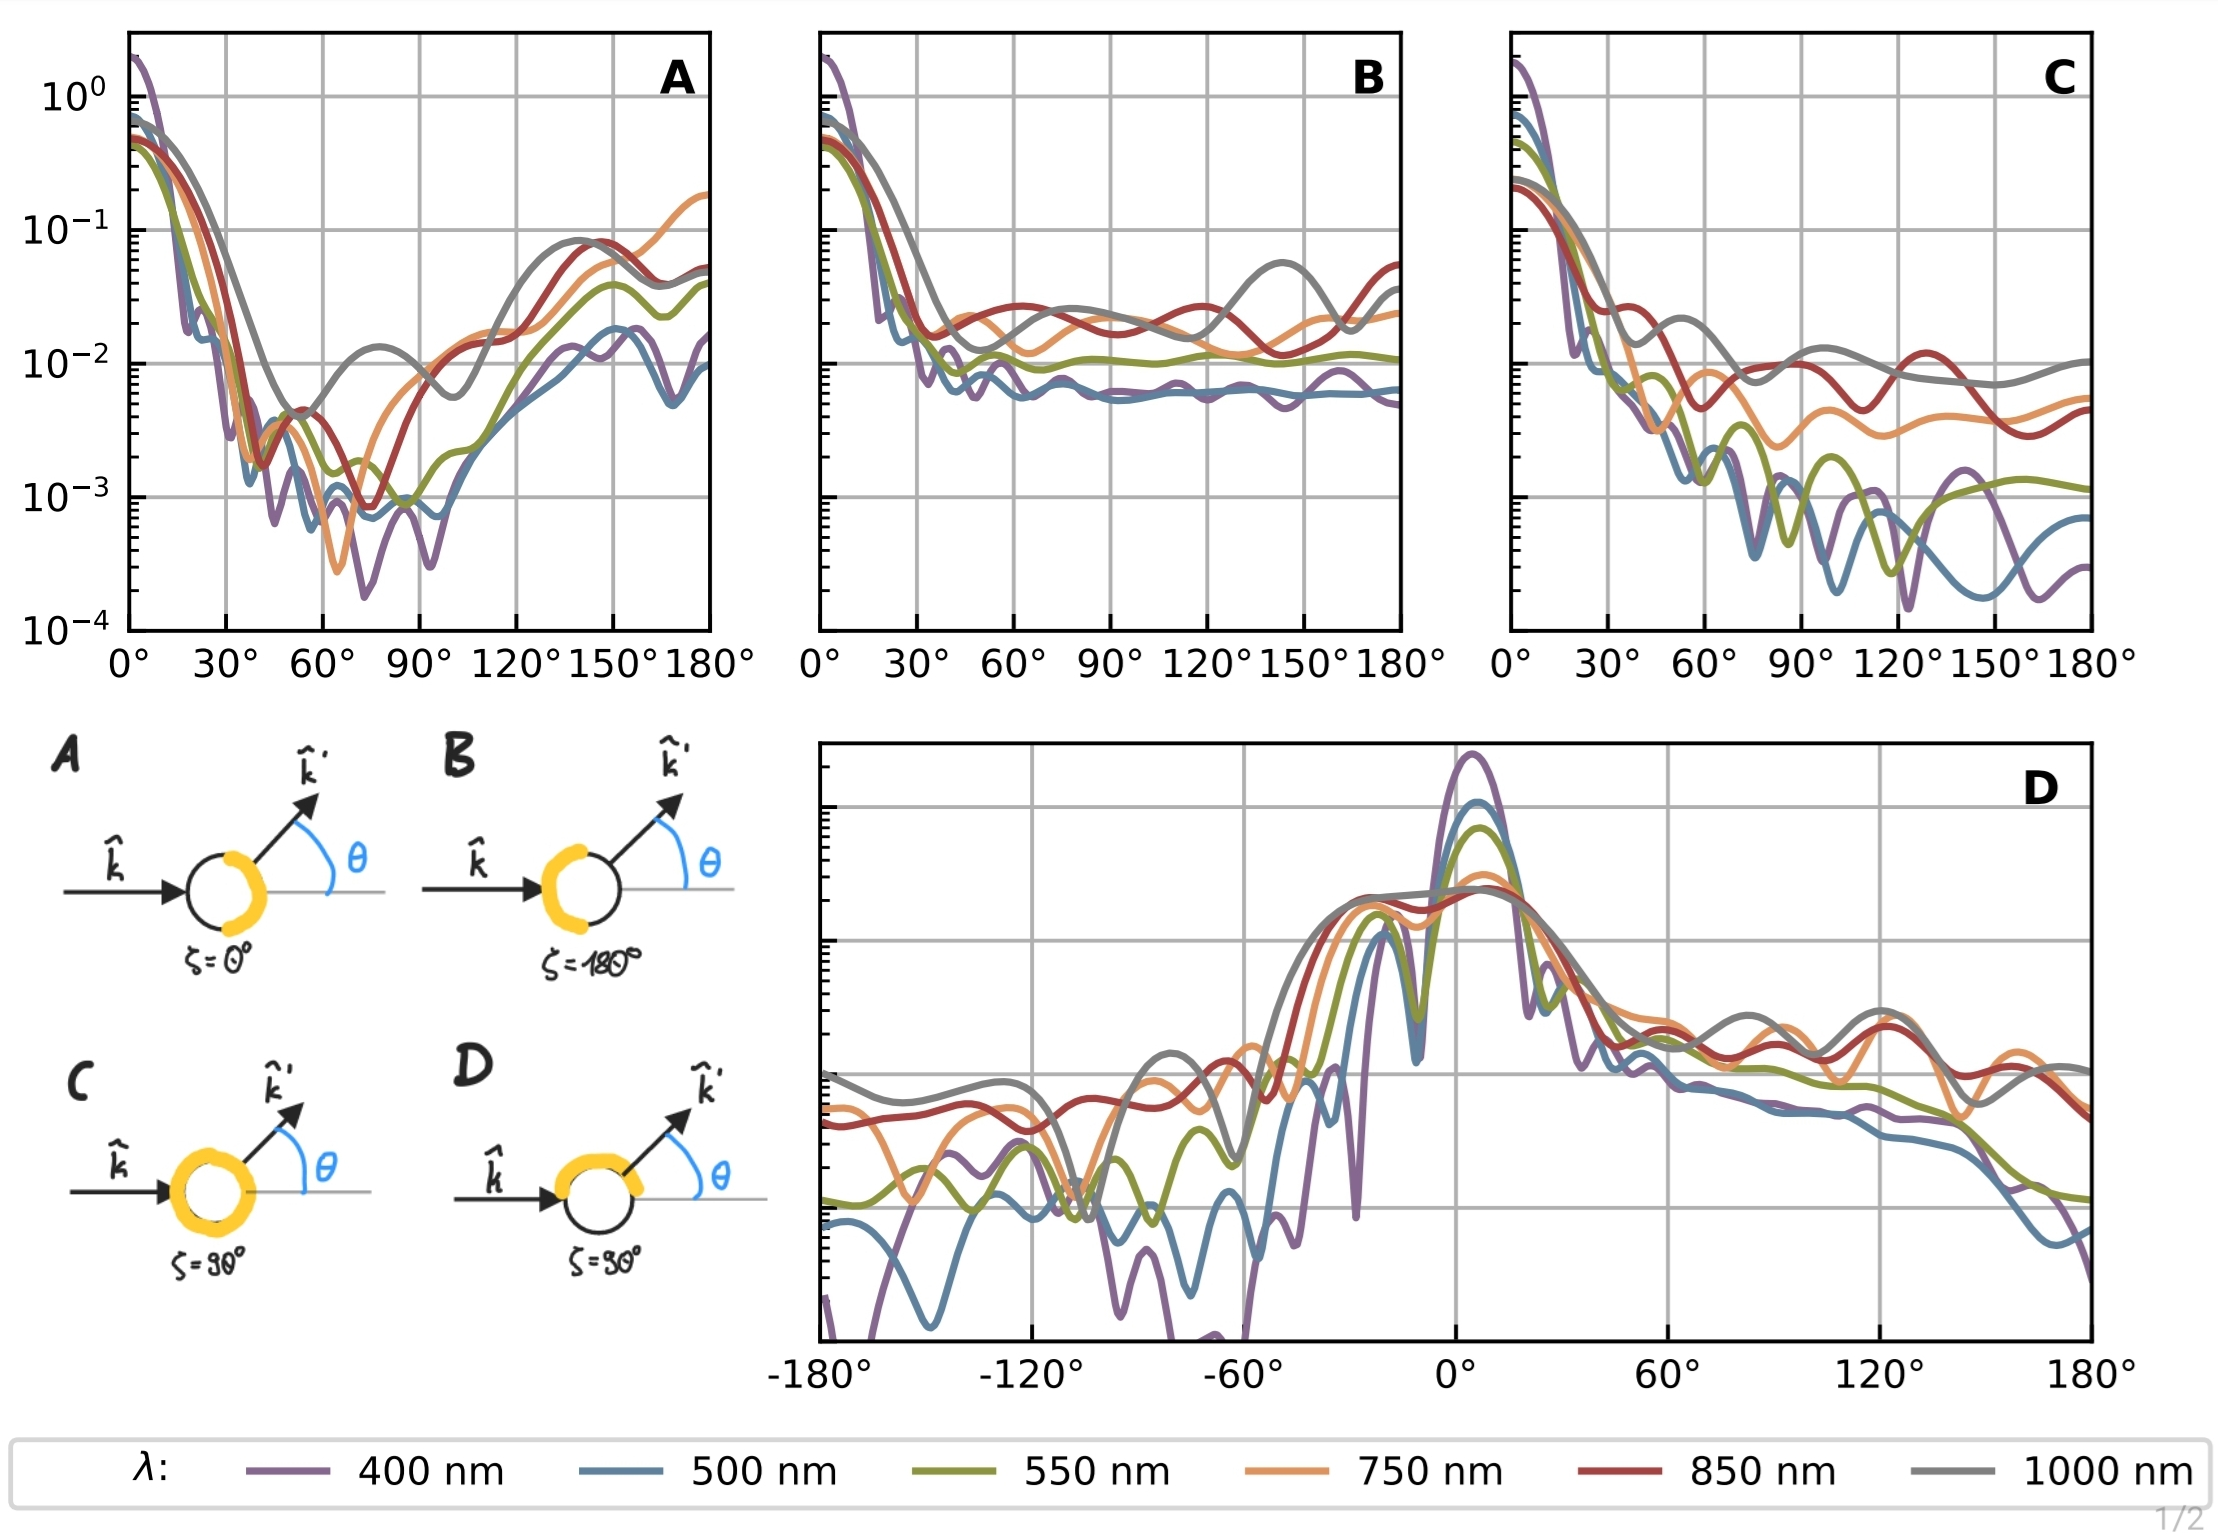
\includegraphics[width=\textwidth]{[fig] cartesian mieplots (placeholder).jpg}
%    \caption{Scattering intensity of the JP versus scattering angle. 
%    {\sffamily\bfseries A} and {\sffamily\bfseries B} show the cylindrically symmetric cases of illumination from the PS side and from the Au side, respectively, i.e. where $\hat{k}\parallel\hat{z}$. 
%    In {\sffamily\bfseries C} and {\sffamily\bfseries D}, the light is incident side-on ($\hat{k}\perp\hat{z}$, $\zeta=\pi/2$).
%    The scattering intensities are taken from the $(\hat{k},\hat{y})$ plane in {\sffamily\bfseries C} (note, that the system is still symmetric under inversion of $y$) and from the $(\hat{k},\hat{z})$ plane, where spatial symmetry is entirely broken, in {\sffamily\bfseries D}.
%    Here, the Au side lies in the positive $\theta$ direction.  
%    }
%    \label{fig:jp-mieplots}
%\end{figure*}


\end{document}
